% Provenance (never printed): see sources/outline_sources.md (Year 1:
% astronomy of position, spherical trigonometry, time scales, insolation).
% Spherical trigonometry is absent from the mathematics series: this chapter
% owns it. Curves computed in figdata/bachelor-1/{sun_paths, day_length,
% celestial_sphere, spherical_triangle}.py (shared model _solar.py); numbers
% of the exercises and problem in the Book 3 scratch calculator ch01.py.
\chapter{Astronomía esférica}\label{ch:b1:spherical-astronomy}

En una noche despejada, lejos de cualquier población, una cámara de larga
exposición apuntada al cielo registra las estrellas como arcos de círculos,
todos centrados en un punto que no se mueve. Una estrella que salió por el este
a las nueve de esta noche saldrá hacia las nueve menos cinco de mañana, y cada
noche algo antes. El Sol al mediodía está más alto en junio que en diciembre, y
en el extremo norte no se pone en pleno verano. Todo esto es la rotación de la
Tierra y su órbita alrededor del Sol, vistas desde el suelo. Para describirlo,
el astrónomo y el geocientífico necesitan coordenadas sobre una esfera, la
trigonometría de los triángulos trazados sobre una esfera y relojes que sigan
el paso de las estrellas o del Sol. Este capítulo construye esas herramientas.
Volverán a aparecer en la cinemática de placas
(\cref{ch:b1:plate-kinematics}), donde las placas giran sobre la esfera, y en
los capítulos sobre el clima (\cref{ch:b1:radiation-heat-transport}), donde la
luz solar que recibe cada \omterm{def:b1:spherical-astronomy:geographic}{latitud} impulsa los vientos y las corrientes.

\begin{recall}
La Tierra gira sobre su eje una vez al día y da una vuelta al Sol una vez al
año, en una órbita casi circular; su eje está inclinado respecto de la órbita,
lo que produce las estaciones (los libros de física de los años 6 y 12; las
leyes de Kepler se recuerdan del libro 3, primer año). Un punto de la Tierra
queda determinado por su \omterm{def:b1:spherical-astronomy:geographic}{latitud} y su longitud (libro 1, año 6). Un vector de
longitud uno queda fijado por dos ángulos, como en las coordenadas esféricas;
el producto escalar de dos vectores unitarios es el coseno del ángulo que
forman, y el producto mixto $\vec u\cdot(\vec v\times\vec w)$ no cambia si se
permutan cíclicamente los tres vectores.
\end{recall}

\section{Triángulos sobre una esfera}

\begin{definition}[Círculo máximo, triángulo esférico]\label{def:b1:spherical-astronomy:spherical-triangle}
Un \emph{círculo máximo}\index{círculo máximo} de una esfera es su intersección
con un plano que pasa por su centro; cualquier otra sección plana es un
\emph{círculo menor}\index{círculo menor}. Por dos puntos que no son
diametralmente opuestos pasa exactamente un círculo máximo, y el más corto de
sus dos arcos es el camino más corto sobre la esfera entre los puntos. Un
\emph{triángulo esférico}\index{triángulo esférico} es la figura formada por tres
puntos de la esfera, sus vértices $A$, $B$, $C$, unidos por arcos de círculos
máximos de menos de \ang{180}. Sus lados $a$, $b$, $c$ (opuestos a $A$, $B$,
$C$) se miden por los ángulos que subtienden en el centro; sus ángulos $A$,
$B$, $C$ son los ángulos entre los planos de los lados que se encuentran en
cada vértice.
\end{definition}

En la esfera de radio $R$, un lado de $a$ radianes mide $Ra$. Todo lado y todo
ángulo están comprendidos entre $0$ y $\pi$.

\begin{omfigure}
\begin{tikzpicture}
\begin{axis}[x=1cm, y=1cm, hide axis, xmin=-2.7, xmax=2.7, ymin=-2.6, ymax=2.6, clip=false]
\draw[black, line width=0.6pt] (axis cs:0,0) circle (2.4cm);
\addplot[black!45, densely dashed, line width=0.4pt] coordinates {(0,0) (-0.078358,1.7847)};
\addplot[black!45, densely dashed, line width=0.4pt] coordinates {(0,0) (-1.5903,-0.2902)};
\addplot[black!45, densely dashed, line width=0.4pt] coordinates {(0,0) (1.4453,-0.16381)};
\addplot[omDef, line width=1.1pt] table {figdata/out/bachelor-1-spherical_triangle-ab.dat};
\addplot[omDef, line width=1.1pt] table {figdata/out/bachelor-1-spherical_triangle-bc.dat};
\addplot[omDef, line width=1.1pt] table {figdata/out/bachelor-1-spherical_triangle-ca.dat};
\addplot[omThm, line width=0.8pt] table {figdata/out/bachelor-1-spherical_triangle-angA.dat};
\addplot[only marks, mark=*, mark size=1.4pt] table[x=x, y=y] {figdata/out/bachelor-1-spherical_triangle-verts.dat};
\fill (axis cs:0,0) circle (1.2pt);
\begin{scope}[font=\small]
  \node[above] at (axis cs:-0.078358,1.7847) {$A$};
  \node[left] at (axis cs:-1.5903,-0.2902) {$B$};
  \node[right] at (axis cs:1.4453,-0.16381) {$C$};
  \node[above left] at (axis cs:0,0) {$O$};
  \node[omThm] at (axis cs:0.24,1.36) {$A$};
  \node[omDef] at (axis cs:0.0,-0.52) {$a$};
  \node[omDef] at (axis cs:0.95,0.95) {$b$};
  \node[omDef] at (axis cs:-1.05,0.95) {$c$};
\end{scope}
\end{axis}
\end{tikzpicture}

{\small Un \omterm{def:b1:spherical-astronomy:spherical-triangle}{triángulo esférico} $ABC$ sobre una esfera de centro $O$. Los lados
$a$, $b$, $c$ son arcos de \omterm{def:b1:spherical-astronomy:spherical-triangle}{círculos máximos}, medidos por los ángulos $BOC$,
$COA$, $AOB$; el ángulo $A$ (rojo) es el ángulo entre los dos lados que se
encuentran en $A$. El triángulo dibujado tiene $a = \ang{78.6}$, $b = \ang{62.6}$,
$c = \ang{64.8}$ y ángulos de \ang{89.9}, \ang{64.9} y \ang{67.4}, que suman más
de \ang{180}.}
\end{omfigure}

\begin{theorem}[Teorema del coseno]\label{thm:b1:spherical-astronomy:cosine-rule}
En un \omterm{def:b1:spherical-astronomy:spherical-triangle}{triángulo esférico},
\[
  \cos a = \cos b\cos c + \sin b\sin c\cos A .
\]
\end{theorem}

\begin{proof}
Trabajemos sobre la esfera unitaria y elijamos los ejes con $A$ en el polo:
$\vec A = (0, 0, 1)$, y el plano $xz$ que contiene a $B$:
$\vec B = (\sin c, 0, \cos c)$, pues $B$ está a la distancia angular $c$ de
$A$. El punto $C$ está a la distancia angular $b$ de $A$, sobre un \omterm{def:b1:spherical-astronomy:spherical-triangle}{círculo
máximo} que pasa por $A$ y forma el ángulo $A$ con el plano $xz$:
$\vec C = (\sin b\cos A, \sin b\sin A, \cos b)$. El lado $a$ es el ángulo entre
$\vec B$ y $\vec C$, así que
\[
  \cos a = \vec B\cdot\vec C = \sin c\sin b\cos A + \cos c\cos b. \qedhere
\]
\end{proof}

\begin{theorem}[Teorema del seno]\label{thm:b1:spherical-astronomy:sine-rule}
En un \omterm{def:b1:spherical-astronomy:spherical-triangle}{triángulo esférico},
\[
  \frac{\sin A}{\sin a} = \frac{\sin B}{\sin b} = \frac{\sin C}{\sin c}.
\]
\end{theorem}

\begin{proof}
Con los vectores de la demostración anterior, el producto vectorial
$\vec B \times \vec C = (-\cos c\sin b\sin A,\ \cos c\sin b\cos A - \sin c\cos b,\
\sin c\sin b\sin A)$, así que el producto mixto es
$\vec A\cdot(\vec B\times\vec C) = \sin b\sin c\sin A$. El producto mixto no cambia
al permutar cíclicamente $A$, $B$, $C$; colocando $B$, y luego $C$, en el polo se
obtiene de la misma manera $\sin c\sin a\sin B$ y $\sin a\sin b\sin
C$. Las tres expresiones son iguales; dividiendo por $\sin a\sin b\sin c$ se
obtiene la regla.
\end{proof}

Cuando los lados son pequeños comparados con el radio, $\cos a \approx 1 -
a^2/2$ y $\sin a \approx a$, y las dos reglas se convierten en las del coseno y
del seno de los triángulos planos: sobre un trozo de esfera lo bastante pequeño
la esfera es plana. En un triángulo grande, en cambio, no es así: los ángulos de
un \omterm{def:b1:spherical-astronomy:spherical-triangle}{triángulo esférico} suman más de \ang{180} (\cref{exo:b1:spherical-astronomy:12}).

\begin{method}[Distancia y rumbo sobre la esfera]\label{met:b1:spherical-astronomy:great-circle}
Para hallar la distancia más corta entre dos lugares de \omterm{def:b1:spherical-astronomy:geographic}{latitudes} $\varphi_1$,
$\varphi_2$ y \omterm{def:b1:spherical-astronomy:geographic}{longitudes} $\lambda_1$, $\lambda_2$, y la dirección en la que
partir:
\begin{enumerate}
  \item forme el triángulo con vértices en el polo norte $P$ y en los dos
        lugares; sus lados desde el polo son las colatitudes $\ang{90} -
        \varphi_1$ y $\ang{90} - \varphi_2$, y su ángulo en el polo es la
        diferencia de \omterm{def:b1:spherical-astronomy:geographic}{longitud} $\Delta\lambda$;
  \item el teorema del coseno da la distancia angular $\Delta$:
        $\cos\Delta = \sin\varphi_1\sin\varphi_2 +
        \cos\varphi_1\cos\varphi_2\cos\Delta\lambda$; la distancia es
        $R\Delta$ ($\Delta$ en radianes);
  \item el rumbo inicial es el ángulo del triángulo en el primer lugar, obtenido
        con el teorema del coseno aplicado al lado opuesto,
        $\sin\varphi_2 = \sin\varphi_1\cos\Delta + \cos\varphi_1\sin\Delta\cos
        \mathrm{Az}$, y se mide desde el norte hacia el segundo lugar.
\end{enumerate}
El rumbo cambia a lo largo del \omterm{def:b1:spherical-astronomy:spherical-triangle}{círculo máximo} (salvo sobre un meridiano o el
ecuador): un barco o un avión que mantenga el mismo rumbo de brújula sigue otra
curva, más larga.
\end{method}

\section{Coordenadas sobre la esfera}

\begin{definition}[Latitud y longitud]\label{def:b1:spherical-astronomy:geographic}
Sea la Tierra una esfera que gira alrededor de su eje polar. La
\emph{latitud}\index{latitud} $\varphi$ de un punto es el ángulo entre el plano
ecuatorial y el radio que pasa por el punto, desde \ang{-90} (polo sur) hasta
\ang{+90} (polo norte); su \emph{longitud}\index{longitud} $\lambda$ es el ángulo,
medido en el plano ecuatorial, entre el semiplano meridiano del punto y el del
meridiano de referencia, el que pasa por Greenwich, contado positivo hacia el
este, desde \ang{-180} hasta \ang{180}.
\end{definition}

De hecho la Tierra está un poco aplastada; la \omterm{def:b1:spherical-astronomy:geographic}{latitud} que se usa en los mapas y
en el cielo es el ángulo entre la vertical local y el plano ecuatorial, que
difiere del ángulo geocéntrico en a lo sumo \ang{0.2}
(\cref{ch:b1:isostasy-gravity}). Las líneas de igual \omterm{def:b1:spherical-astronomy:geographic}{latitud}, los paralelos, son
\omterm{def:b1:spherical-astronomy:spherical-triangle}{círculos menores}; los meridianos son mitades de \omterm{def:b1:spherical-astronomy:spherical-triangle}{círculos máximos}.

\begin{definition}[La esfera celeste]\label{def:b1:spherical-astronomy:celestial-sphere}
La \emph{esfera celeste}\index{esfera celeste} es una esfera imaginaria centrada
en el observador, sobre la que cada estrella se sitúa en su dirección; solo
importan las direcciones, no las distancias. Las prolongaciones del eje de la
Tierra cortan a la esfera en los \emph{polos celestes}\index{polo celeste} norte
y sur; el plano del ecuador terrestre la corta según el \emph{ecuador
celeste}\index{ecuador celeste}. El \emph{cenit}\index{cenit} es el punto situado
justo encima, sobre la vertical del lugar; el horizonte es el \omterm{def:b1:spherical-astronomy:spherical-triangle}{círculo máximo} a
$\ang{90}$ de él. El \emph{meridiano local}\index{meridiano local} es el \omterm{def:b1:spherical-astronomy:spherical-triangle}{círculo
máximo} que pasa por el cenit y por los polos celestes; corta al horizonte en los
puntos norte y sur.
\end{definition}

Al girar la Tierra de oeste a este, la \omterm{def:b1:spherical-astronomy:celestial-sphere}{esfera celeste} parece girar en sentido
contrario, de este a oeste, alrededor del eje de los \omterm{def:b1:spherical-astronomy:celestial-sphere}{polos celestes}, una vuelta
en algo menos de un día. Las estrellas conservan sus posiciones relativas: están
tan lejos que un viaje de un año alrededor del Sol cambia sus direcciones en
menos de un segundo de arco (\cref{ch:b1:observing-the-sky}).

\begin{definition}[Coordenadas horizontales]\label{def:b1:spherical-astronomy:horizontal}
La \emph{altura}\index{altura (de un astro)} $h$ de una estrella es su ángulo
sobre el horizonte, desde \ang{-90} hasta \ang{90}; su distancia cenital es
$z = \ang{90} - h$. Su \emph{acimut}\index{acimut} $\mathrm{A}$ es el ángulo, a
lo largo del horizonte, desde el punto norte hasta el pie del círculo vertical
de la estrella, contado de \ang{0} a \ang{360} pasando por el este.
\end{definition}

Las coordenadas horizontales son las del observador: cambian con el lugar y con
el tiempo. Las coordenadas del propio cielo se mueven con su rotación.

\begin{definition}[Coordenadas ecuatoriales]\label{def:b1:spherical-astronomy:equatorial}
La \emph{declinación}\index{declinación (celeste)} $\delta$ de una estrella es su
ángulo respecto del \omterm{def:b1:spherical-astronomy:celestial-sphere}{ecuador celeste}, positivo hacia el norte, desde \ang{-90}
hasta \ang{90}. El \omterm{def:b1:spherical-astronomy:spherical-triangle}{círculo máximo} que pasa por la estrella y por los \omterm{def:b1:spherical-astronomy:celestial-sphere}{polos
celestes} es su círculo horario. El \emph{ángulo horario}\index{ángulo horario} $H$
de la estrella es el ángulo, en el \omterm{def:b1:spherical-astronomy:celestial-sphere}{polo celeste}, entre el \omterm{def:b1:spherical-astronomy:celestial-sphere}{meridiano local} y el
círculo horario de la estrella, contado hacia el oeste, en horas de \ang{15}. La
\emph{ascensión recta}\index{ascensión recta} $\alpha$ es el ángulo a lo largo del
\omterm{def:b1:spherical-astronomy:celestial-sphere}{ecuador celeste} desde un punto fijo del cielo, el \omterm{def:b1:spherical-astronomy:ecliptic}{punto vernal}
(\cref{def:b1:spherical-astronomy:ecliptic}), hasta el círculo horario de la
estrella, contado hacia el este, también en horas.
\end{definition}

La \omterm{def:b1:spherical-astronomy:equatorial}{declinación} y la \omterm{def:b1:spherical-astronomy:equatorial}{ascensión recta} son fijas en el cielo, como la \omterm{def:b1:spherical-astronomy:geographic}{latitud} y la
longitud en la Tierra: los catálogos las recogen. La palabra \omterm{def:b1:spherical-astronomy:equatorial}{declinación} se usa
aquí solo en este sentido astronómico; el ángulo entre el norte geográfico y el
norte de una brújula se llama siempre declinación magnética
(\cref{ch:b1:field-lab-methods-1}).

\begin{proposition}[De coordenadas ecuatoriales a horizontales]\label{prop:b1:spherical-astronomy:transform}
A la \omterm{def:b1:spherical-astronomy:geographic}{latitud} $\varphi$, una estrella de \omterm{def:b1:spherical-astronomy:equatorial}{declinación} $\delta$ y \omterm{def:b1:spherical-astronomy:equatorial}{ángulo horario} $H$
tiene la \omterm{def:b1:spherical-astronomy:horizontal}{altura} y el \omterm{def:b1:spherical-astronomy:horizontal}{acimut} dados por
\[
  \sin h = \sin\varphi\sin\delta + \cos\varphi\cos\delta\cos H,
  \qquad
  \cos\mathrm{A} = \frac{\sin\delta - \sin\varphi\sin h}{\cos\varphi\cos h},
\]
con $\mathrm{A}$ comprendido entre \ang{0} y \ang{180} cuando la estrella está al
este del meridiano ($\sin H < 0$) y $\mathrm{A} = \ang{360} - \arccos(\dots)$
cuando está al oeste. En particular, la \omterm{def:b1:spherical-astronomy:horizontal}{altura} del \omterm{def:b1:spherical-astronomy:celestial-sphere}{polo celeste} norte es igual a
la \omterm{def:b1:spherical-astronomy:geographic}{latitud}.
\end{proposition}

\begin{proof}
Consideremos el triángulo formado por el \omterm{def:b1:spherical-astronomy:celestial-sphere}{polo celeste} norte $P$, el \omterm{def:b1:spherical-astronomy:celestial-sphere}{cenit} $Z$ y
la estrella $X$ (el triángulo de posición, o astronómico). La vertical local forma
el ángulo $\varphi$ con el plano ecuatorial, así que $PZ =
\ang{90} - \varphi$;
$PX = \ang{90} - \delta$; $ZX = \ang{90} - h$. El ángulo en $P$ es el \omterm{def:b1:spherical-astronomy:equatorial}{ángulo
horario} $H$; el ángulo en $Z$ es el \omterm{def:b1:spherical-astronomy:horizontal}{acimut} de la estrella medido desde el norte
(al este o al oeste del meridiano). El teorema del coseno para el lado $ZX$, opuesto
a $P$, da
$\cos(\ang{90} - h) = \cos(\ang{90} - \varphi)\cos(\ang{90} - \delta) +
\sin(\ang{90} - \varphi)\sin(\ang{90} - \delta)\cos H$, la primera fórmula.
El teorema del coseno para el lado $PX$, opuesto a $Z$, da
$\sin\delta = \sin\varphi\sin h + \cos\varphi\cos h\cos\mathrm{A}$, la
segunda. Para el polo, $\delta = \ang{90}$ y la primera fórmula se reduce a
$\sin h = \sin\varphi$.
\end{proof}

\begin{omfigure}
\begin{tikzpicture}
\pic (cs) at (0,0) {celestialsphere=45};
\begin{axis}[x=1cm, y=1cm, hide axis, anchor=origin, at={(0,0)}, xmin=-2.6, xmax=2.6, ymin=-2.4, ymax=2.5, clip=false]
\addplot[omField, line width=1.1pt] table[x=x, y=y] {figdata/out/bachelor-1-celestial_sphere-vertical.dat};
\addplot[black!80, line width=0.9pt, densely dash dot] table[x=x, y=y] {figdata/out/bachelor-1-celestial_sphere-hourcircle.dat};
\addplot[only marks, mark=star, mark size=3pt, mark options={line width=0.8pt}] table[x=x, y=y] {figdata/out/bachelor-1-celestial_sphere-star.dat};
\end{axis}
\begin{scope}[font=\footnotesize]
  \node[above] at (cs-Z) {$Z$};
  \node[above left] at (cs-NCP) {$P$};
  \node[left] at (cs-N) {N};
  \node[right] at (cs-S) {S};
  \node[below] at (cs-W) {O};
  \node[below, fill=white, fill opacity=0.8, text opacity=1, inner sep=1pt] at (cs-E) {E};
  \node[above right] at (0.2262,0.94) {$X$};
  \node[omField] at (0.55,0.2) {$h$};
  \node[omDef, right] at (2.0,-1.25) {ecuador};
  \node[left] at (-2.0,-0.3) {horizonte};
  \node at (-1.35,0.62) {$\varphi$};
\end{scope}
\draw[black!60, line width=0.4pt] (-1.05,0) arc[start angle=180, end angle=137, radius=1.05cm];
\end{tikzpicture}

{\small El cielo a la \omterm{def:b1:spherical-astronomy:geographic}{latitud} \ang{45} N, visto desde el oeste, con el norte a la
izquierda. El \omterm{def:b1:spherical-astronomy:celestial-sphere}{polo celeste} norte $P$ está a una \omterm{def:b1:spherical-astronomy:horizontal}{altura} sobre el punto norte igual
a la \omterm{def:b1:spherical-astronomy:geographic}{latitud} (en rojo: el eje de los \omterm{def:b1:spherical-astronomy:celestial-sphere}{polos celestes}); el \omterm{def:b1:spherical-astronomy:celestial-sphere}{ecuador celeste} (azul)
corta al horizonte en los puntos este y oeste. Una estrella $X$ de \omterm{def:b1:spherical-astronomy:equatorial}{declinación}
\ang{25}, tres horas y veinte minutos después de su paso por el meridiano (\omterm{def:b1:spherical-astronomy:equatorial}{ángulo
horario} \ang{50}), está a la \omterm{def:b1:spherical-astronomy:horizontal}{altura} $h = \ang{45.3}$ (en verde: su círculo
vertical, desde el \omterm{def:b1:spherical-astronomy:celestial-sphere}{cenit} $Z$ hasta el horizonte) y al \omterm{def:b1:spherical-astronomy:horizontal}{acimut} \ang{261}; su círculo
horario (trazo y punto) va desde el polo hasta el ecuador pasando por la estrella.
Calculado con \cref{prop:b1:spherical-astronomy:transform}.}
\end{omfigure}

\begin{proposition}[Culminación y estrellas circumpolares]\label{prop:b1:spherical-astronomy:culmination}
A la \omterm{def:b1:spherical-astronomy:geographic}{latitud} $\varphi$, una estrella de \omterm{def:b1:spherical-astronomy:equatorial}{declinación} $\delta$ cruza el meridiano
($H = 0$) a la \omterm{def:b1:spherical-astronomy:horizontal}{altura} $\ang{90} - |\varphi - \delta|$, al sur del \omterm{def:b1:spherical-astronomy:celestial-sphere}{cenit} si
$\delta < \varphi$, al norte de él si $\delta > \varphi$. En el hemisferio norte
($\varphi > 0$) nunca se pone si $\delta > \ang{90} - \varphi$ y nunca sale si
$\delta < -(\ang{90} - \varphi)$.
\end{proposition}

\begin{proof}
Para $H = 0$, $\sin h = \sin\varphi\sin\delta + \cos\varphi\cos\delta =
\cos(\varphi - \delta)$, luego $h = \ang{90} - |\varphi - \delta|$. La \omterm{def:b1:spherical-astronomy:horizontal}{altura}
mínima, en $H = \ang{180}$, cumple $\sin h = -\cos(\varphi + \delta)$; es positiva
cuando $\varphi + \delta > \ang{90}$. La estrella permanece bajo el horizonte cuando
incluso su \omterm{def:b1:spherical-astronomy:horizontal}{altura} máxima es negativa, $|\varphi - \delta| > \ang{90}$.
\end{proof}

\begin{definition}[Estrella circumpolar]\label{def:b1:spherical-astronomy:circumpolar}
Una \emph{estrella circumpolar}\index{estrella circumpolar} es una estrella que
nunca se pone a la \omterm{def:b1:spherical-astronomy:geographic}{latitud} del observador: da vueltas alrededor del \omterm{def:b1:spherical-astronomy:celestial-sphere}{polo celeste},
cruza el meridiano por encima del polo y, doce horas sidéreas después, por debajo.
\end{definition}

\begin{omfigure}
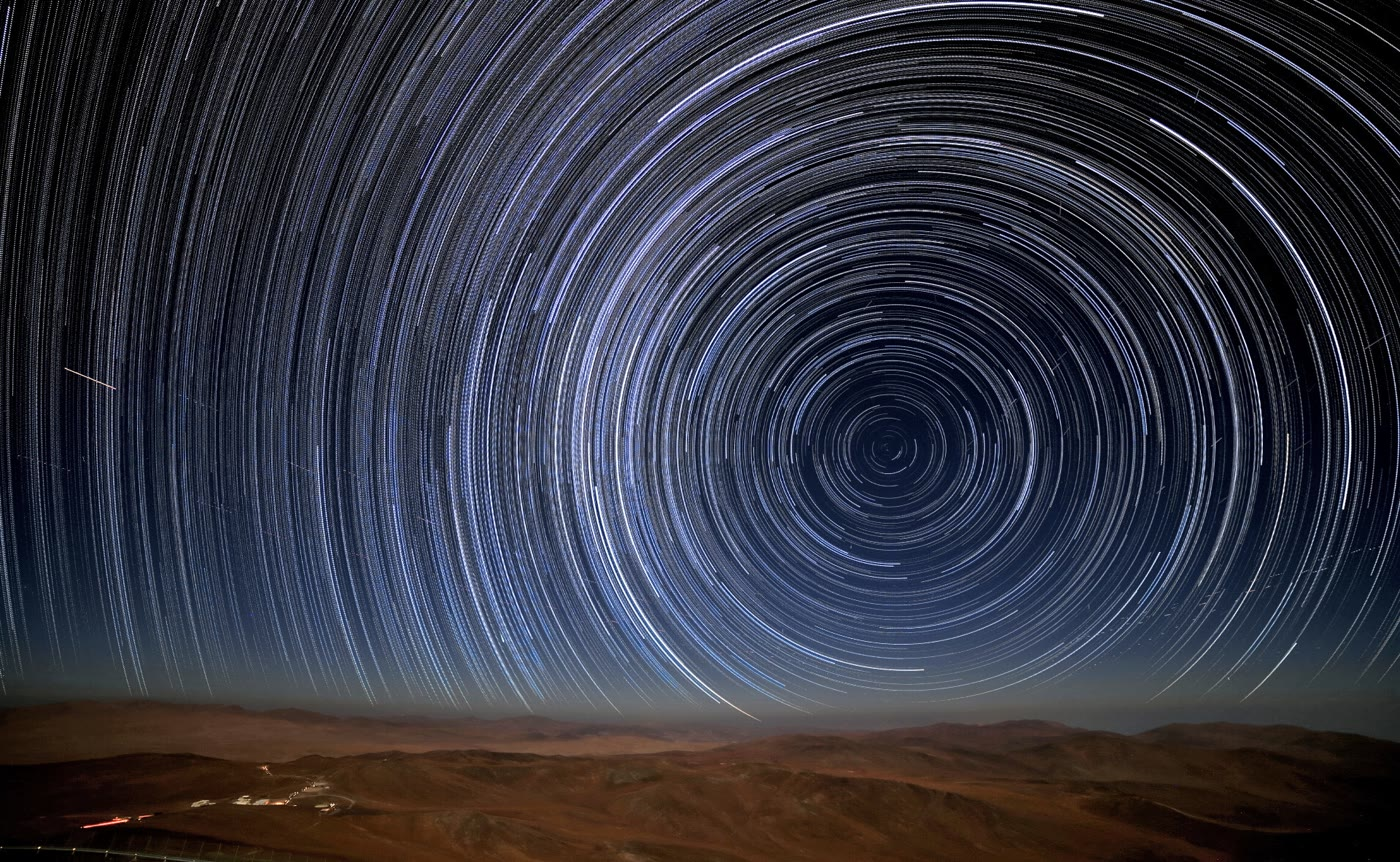
\includegraphics[width=0.8\linewidth]{images/book3/b1-star-trails-paranal.jpg}
% ledger: commons:eso-paranal-star-trails, mpc:paranal

{\small Trazos de estrellas sobre el Observatorio de Paranal, en el desierto de
Atacama, a la \omterm{def:b1:spherical-astronomy:geographic}{latitud} \ang{24.6} S: una exposición larga registra el arco de cada
estrella alrededor del \omterm{def:b1:spherical-astronomy:celestial-sphere}{polo celeste} sur, que se encuentra \ang{24.6} sobre el
horizonte sur. Fotografía de R.~Wesson/ESO, CC BY 4.0.}
\end{omfigure}

\section{Tiempo sidéreo y tiempo solar}

\begin{definition}[La eclíptica]\label{def:b1:spherical-astronomy:ecliptic}
La \emph{eclíptica}\index{eclíptica} es el \omterm{def:b1:spherical-astronomy:spherical-triangle}{círculo máximo} de la \omterm{def:b1:spherical-astronomy:celestial-sphere}{esfera celeste}
sobre el que el Sol parece moverse en un año, la traza del plano de la órbita de
la Tierra. Está inclinada respecto del \omterm{def:b1:spherical-astronomy:celestial-sphere}{ecuador celeste} en la
\emph{oblicuidad de la eclíptica}\index{oblicuidad de la eclíptica} $\varepsilon$,
la inclinación del eje de la Tierra respecto de su órbita. La eclíptica corta al
ecuador en dos puntos; el \emph{punto vernal}\index{punto vernal} $\gamma$ es aquel
en el que el Sol cruza el ecuador hacia el norte, en marzo. La longitud eclíptica
del Sol $\lambda_\odot$ es su ángulo a lo largo de la eclíptica desde $\gamma$,
contado hacia el este.
\end{definition}

% ledger: earth:obliquity (23.44)
La oblicuidad es hoy $\varepsilon = \ang{23.44}$.

\begin{definition}[Tiempo sidéreo]\label{def:b1:spherical-astronomy:sidereal-time}
El \emph{tiempo sidéreo}\index{tiempo sidéreo} local es el \omterm{def:b1:spherical-astronomy:equatorial}{ángulo horario} del \omterm{def:b1:spherical-astronomy:ecliptic}{punto
vernal} $\gamma$. Un día sidéreo es el intervalo entre dos pasos de $\gamma$ por el
meridiano.
\end{definition}

Como la \omterm{def:b1:spherical-astronomy:equatorial}{ascensión recta} se cuenta hacia el este desde $\gamma$ y el \omterm{def:b1:spherical-astronomy:equatorial}{ángulo horario}
hacia el oeste desde el meridiano, para cada estrella
\[
  H = \mathrm{LST} - \alpha ,
\]
donde LST es el \omterm{def:b1:spherical-astronomy:sidereal-time}{tiempo sidéreo} local: una estrella cruza el meridiano cuando el
\omterm{def:b1:spherical-astronomy:sidereal-time}{tiempo sidéreo} es igual a su \omterm{def:b1:spherical-astronomy:equatorial}{ascensión recta}. Un reloj de observatorio que marque
el \omterm{def:b1:spherical-astronomy:sidereal-time}{tiempo sidéreo} indica de un vistazo qué parte del cielo está en el \omterm{def:b1:spherical-astronomy:celestial-sphere}{cenit}.

\begin{proposition}[Días sidéreo y solar]\label{prop:b1:spherical-astronomy:sidereal-day}
En un \omterm{def:b1:spherical-astronomy:tropical-year}{año trópico} de $N$ días solares medios, la Tierra da $N + 1$ vueltas
respecto de las estrellas. Por tanto, el día sidéreo dura
\[
  \frac{N}{N + 1}\times\qty{24}{h},
\]
y con $N = 365.2422$ esto da \qty{23}{h}~\qty{56}{min}~\qty{4.09}{s}: una estrella
cruza el meridiano \qty{3}{min}~\qty{56}{s} de \omterm{def:b1:spherical-astronomy:solar-time}{tiempo solar medio} antes cada día.
\end{proposition}

\begin{proof}
% ledger: usno:tropical-year, earth:Trot (23.9345 h)
Contemos las vueltas respecto del Sol y respecto de las estrellas a lo largo de un
año. El Sol da una vuelta a la \omterm{def:b1:spherical-astronomy:ecliptic}{eclíptica} hacia el este en un año, en el sentido de
la rotación de la Tierra. Respecto del Sol, la Tierra da, pues, una vuelta menos
que respecto de las estrellas: $N$ días solares y $N + 1$ días sidéreos llenan el
mismo año. El día sidéreo es $N/(N+1)$ de un día solar, es decir,
$\qty{86400}{s}\times 365.2422/366.2422 = \qty{86164.09}{s}$; la diferencia es
$\qty{235.9}{s}$. Esto concuerda con el periodo de rotación de la Tierra respecto de
las estrellas, \qty{23.9345}{h}.
\end{proof}

\begin{definition}[Tiempo solar]\label{def:b1:spherical-astronomy:solar-time}
El \emph{tiempo solar aparente}\index{tiempo solar aparente} es el \omterm{def:b1:spherical-astronomy:equatorial}{ángulo horario}
del Sol más 12 horas: un reloj de sol lo indica, y es mediodía cuando el Sol cruza
el meridiano. El \emph{tiempo solar medio}\index{tiempo solar medio} es el \omterm{def:b1:spherical-astronomy:equatorial}{ángulo
horario}, más 12 horas, de un Sol ficticio medio que recorre el \omterm{def:b1:spherical-astronomy:celestial-sphere}{ecuador celeste} a
ritmo uniforme, dando una vuelta en un \omterm{def:b1:spherical-astronomy:tropical-year}{año trópico}. Su diferencia, aparente menos
medio, es la \emph{ecuación del tiempo}\index{ecuación del tiempo}.
\end{definition}

El Sol verdadero adelanta y retrasa respecto del Sol medio por dos razones. La
Tierra se mueve más deprisa cerca del perihelio, a comienzos de enero, que cerca
del afelio, así que el avance del Sol a lo largo de la \omterm{def:b1:spherical-astronomy:ecliptic}{eclíptica} es irregular
(segunda ley de Kepler); y el Sol se mueve por la \omterm{def:b1:spherical-astronomy:ecliptic}{eclíptica}, inclinada respecto
del ecuador, de modo que incluso un movimiento uniforme a lo largo de la \omterm{def:b1:spherical-astronomy:ecliptic}{eclíptica}
se proyecta sobre el ecuador, que es lo que mide el \omterm{def:b1:spherical-astronomy:equatorial}{ángulo horario}, de forma
irregular, más deprisa cerca de los solsticios que cerca de los equinoccios. Los
relojes civiles marcan el \omterm{def:b1:spherical-astronomy:solar-time}{tiempo solar medio} del meridiano de referencia de su
huso horario; la hora solar media en la \omterm{def:b1:spherical-astronomy:geographic}{longitud} $\lambda$ va por delante de la
hora de Greenwich en $\lambda/\ang{15}$ horas.

\begin{omfigure}
\begin{tikzpicture}
\begin{axis}[omrecord, width=0.9\linewidth, height=5.2cm, xmin=0, xmax=365,
  xtick={0,31,59,90,120,151,181,212,243,273,304,334,365},
  xticklabels={E,F,M,A,M,J,J,A,S,O,N,D,},
  ylabel={ecuación del tiempo (min)}, ymin=-20, ymax=21,
  tick label style={font=\scriptsize}, label style={font=\small}]
\addplot[black!50, line width=0.4pt] coordinates {(0,0) (365,0)};
\addplot[omDef, line width=1.1pt] table[x=day, y=eot_min] {figdata/out/bachelor-1-day_length-eot.dat};
\node[font=\scriptsize, above, fill=white, inner sep=1pt] at (axis cs:306,16.6) {$+16.4$};
\node[font=\scriptsize, below, fill=white, inner sep=1pt] at (axis cs:41,-14.4) {$-14.2$};
\end{axis}
\end{tikzpicture}

{\small La \omterm{def:b1:spherical-astronomy:solar-time}{ecuación del tiempo} a lo largo del año (\omterm{def:b1:spherical-astronomy:solar-time}{tiempo solar aparente} menos
medio): un reloj de sol adelanta hasta \qty{16.4}{min} a comienzos de noviembre y
atrasa \qty{14.2}{min} a mediados de febrero. Calculada con una órbita de Kepler de
excentricidad 0.0167, la oblicuidad \ang{23.44}, la longitud del perihelio y la
fecha del equinoccio de marzo de 2026.}
% ledger: earth:ecc, earth:obliquity, nasa:earth-perihelion-longitude, usno:seasons-2026
\end{omfigure}

\section{Salida, puesta y el Sol}

\begin{proposition}[Salida y puesta]\label{prop:b1:spherical-astronomy:rising}
A la \omterm{def:b1:spherical-astronomy:geographic}{latitud} $\varphi$, una estrella de \omterm{def:b1:spherical-astronomy:equatorial}{declinación} $\delta$ que sale y se pone
cruza el horizonte en los \omterm{def:b1:spherical-astronomy:equatorial}{ángulos horarios} $\pm H_0$ con
\[
  \cos H_0 = -\tan\varphi\tan\delta ,
\]
en el \omterm{def:b1:spherical-astronomy:horizontal}{acimut} $\mathrm{A}_0$ con $\cos\mathrm{A}_0 = \sin\delta/\cos\varphi$
(en la salida; se pone en $\ang{360} - \mathrm{A}_0$). Permanece sobre el horizonte
durante $2H_0$, convertido en horas a razón de \ang{15} por hora.
\end{proposition}

\begin{proof}
En el horizonte $h = 0$, y la \cref{prop:b1:spherical-astronomy:transform} da
$0 = \sin\varphi\sin\delta + \cos\varphi\cos\delta\cos H_0$, y
$\cos\mathrm{A}_0 = \sin\delta/\cos\varphi$. El \omterm{def:b1:spherical-astronomy:equatorial}{ángulo horario} crece uniformemente,
a razón de \ang{15} por hora, desde $-H_0$ en la salida hasta $+H_0$ en la puesta.
\end{proof}

Para el Sol esto da la duración del día, si el Sol se trata como un punto y se
ignora la refracción de la luz por el aire (que añaden unos minutos de luz
diurna). En los equinoccios $\delta = 0$, $H_0 = \ang{90}$: el día y la noche duran
doce horas en todas partes, y el Sol sale exactamente por el este.

\begin{omfigure}
\begin{tikzpicture}
\begin{axis}[omrecord, width=0.85\linewidth, height=5.6cm, xmin=40, xmax=320, ymin=0, ymax=75,
  xtick={45,90,135,180,225,270,315}, xticklabels={NE,E,SE,S,SO,O,NO}, ytick={0,15,30,45,60,75},
  xlabel={acimut}, ylabel={altura del Sol ($^\circ$)},
  tick label style={font=\scriptsize}, label style={font=\small}]
\addplot[omThm, line width=1pt] table[x=az_deg, y=alt_deg] {figdata/out/bachelor-1-sun_paths-june.dat};
\addplot[black, line width=1pt] table[x=az_deg, y=alt_deg] {figdata/out/bachelor-1-sun_paths-equinox.dat};
\addplot[omDef, line width=1pt] table[x=az_deg, y=alt_deg] {figdata/out/bachelor-1-sun_paths-december.dat};
\begin{scope}[font=\scriptsize, fill=white, fill opacity=0.8, text opacity=1, inner sep=1pt]
  \node[omThm, above, fill=white] at (axis cs:180,68.4) {solsticio de junio, $\ang{68.4}$};
  \node[above, fill=white] at (axis cs:180,45) {equinoccios, $\ang{45}$};
  \node[omDef, above, fill=white] at (axis cs:180,21.6) {solsticio de diciembre, $\ang{21.6}$};
\end{scope}
\end{axis}
\end{tikzpicture}

{\small La trayectoria del Sol por el cielo a la \omterm{def:b1:spherical-astronomy:geographic}{latitud} \ang{45} N en el solsticio
de junio (rojo), los equinoccios (negro) y el solsticio de diciembre (azul), con
las \omterm{def:b1:spherical-astronomy:horizontal}{alturas} al mediodía $\ang{90} - \varphi + \delta_\odot$. En los equinoccios el
Sol sale exactamente por el este y se pone por el oeste; en junio sale por el
nordeste.}
\end{omfigure}

\begin{proposition}[Declinación del Sol]\label{prop:b1:spherical-astronomy:sun-declination}
Cuando el Sol está en la \omterm{def:b1:spherical-astronomy:geographic}{longitud} \omterm{def:b1:spherical-astronomy:ecliptic}{eclíptica} $\lambda_\odot$, su \omterm{def:b1:spherical-astronomy:equatorial}{declinación} y su
\omterm{def:b1:spherical-astronomy:equatorial}{ascensión recta} cumplen
\[
  \sin\delta_\odot = \sin\varepsilon\sin\lambda_\odot, \qquad
  \tan\alpha_\odot = \cos\varepsilon\tan\lambda_\odot .
\]
\end{proposition}

\begin{proof}
Tomemos ejes con $x$ hacia $\gamma$ y $z$ hacia el \omterm{def:b1:spherical-astronomy:celestial-sphere}{polo celeste} norte. En los ejes
$x$, $y'$, $z'$ ligados a la \omterm{def:b1:spherical-astronomy:ecliptic}{eclíptica}, con $z'$ hacia su polo, la dirección del
Sol es $(\cos\lambda_\odot, \sin\lambda_\odot, 0)$. Los ejes de la \omterm{def:b1:spherical-astronomy:ecliptic}{eclíptica} son los
del ecuador girados el ángulo $\varepsilon$ alrededor de $x$, así que en los ejes
ecuatoriales la dirección del Sol es
$(\cos\lambda_\odot,\ \sin\lambda_\odot\cos\varepsilon,\
\sin\lambda_\odot\sin\varepsilon)$. Su componente $z$ es $\sin\delta_\odot$; el
cociente de sus componentes $y$ y $x$ es $\tan\alpha_\odot$.
\end{proof}

\begin{omfigure}
\begin{tikzpicture}
\begin{axis}[omrecord, width=0.9\linewidth, height=6cm, xmin=0, xmax=365, ymin=0, ymax=24,
  xtick={0,31,59,90,120,151,181,212,243,273,304,334,365},
  xticklabels={E,F,M,A,M,J,J,A,S,O,N,D,}, ytick={0,6,12,18,24},
  ylabel={duración del día (h)}, tick label style={font=\scriptsize}, label style={font=\small},
  legend style={font=\scriptsize, at={(0.5,1.02)}, anchor=south, draw=none}, legend columns=5,
  legend cell align=left]
\addplot[black, line width=0.9pt] table[x=day, y=lat0] {figdata/out/bachelor-1-day_length-lengths.dat};
\addplot[omDef, line width=0.9pt] table[x=day, y=lat30] {figdata/out/bachelor-1-day_length-lengths.dat};
\addplot[omThm, line width=0.9pt] table[x=day, y=lat45] {figdata/out/bachelor-1-day_length-lengths.dat};
\addplot[omField, line width=0.9pt] table[x=day, y=lat60] {figdata/out/bachelor-1-day_length-lengths.dat};
\addplot[black, line width=0.9pt, densely dashed] table[x=day, y=lat70] {figdata/out/bachelor-1-day_length-lengths.dat};
\legend{\ang{0}, \ang{30} N, \ang{45} N, \ang{60} N, \ang{70} N}
\end{axis}
\end{tikzpicture}

{\small Duración del día (centro del Sol por encima del horizonte geométrico) a lo
largo del año en cinco \omterm{def:b1:spherical-astronomy:geographic}{latitudes} norte, a partir de
\cref{prop:b1:spherical-astronomy:rising,prop:b1:spherical-astronomy:sun-declination}.
A \ang{70} N el Sol se mantiene sobre el horizonte durante semanas alrededor del
solsticio de junio y permanece bajo él alrededor del solsticio de diciembre. En el
hemisferio sur las curvas están desplazadas medio año.}
\end{omfigure}

\begin{definition}[Insolación]\label{def:b1:spherical-astronomy:insolation}
La \emph{insolación}\index{insolación} en un lugar y un instante es la potencia de
la luz solar recibida por unidad de área de una superficie horizontal en el alto de
la atmósfera. Con $S_0$ la irradiancia solar a la distancia media $a$ del Sol, $r$
la distancia real y $\theta_z$ la distancia cenital del Sol,
\[
  I = S_0\left(\frac{a}{r}\right)^{2}\cos\theta_z = S_0\left(\frac{a}{r}\right)^{2}\sin h_\odot
  \quad (h_\odot > 0), \qquad I = 0 \text{ de noche}.
\]
\end{definition}

% ledger: earth:TSI (1361 W/m2), earth:peri, earth:aph, earth:a
El factor $(a/r)^2$ es la ley de la inversa del cuadrado para la luz (los libros de
física); el factor $\cos\theta_z$ aparece porque un haz de sección un metro cuadrado
se extiende sobre $1/\cos\theta_z$ metros cuadrados de suelo horizontal. Con
$S_0 = \qty{1361}{W.m^{-2}}$ y una distancia Sol--Tierra de \qty{147.1e6}{km} en el
perihelio y \qty{152.1e6}{km} en el afelio, el factor $(a/r)^2$ varía en
$\pm\qty{3.4}{\percent}$ a lo largo del año. La inclinación del eje hace mucho más:
cambia a la vez la \omterm{def:b1:spherical-astronomy:horizontal}{altura} del Sol al mediodía y la duración del día, y estas dos
cosas juntas producen las estaciones. Las sumas diarias y anuales de la \omterm{def:b1:spherical-astronomy:insolation}{insolación},
que impulsan el clima, se calculan en el
\cref{ch:b1:radiation-heat-transport}.


\section{Calendarios}

\begin{definition}[Año trópico]\label{def:b1:spherical-astronomy:tropical-year}
El \emph{año trópico}\index{año trópico} es el intervalo medio entre dos pasos del
Sol por el \omterm{def:b1:spherical-astronomy:ecliptic}{punto vernal}. Rige las estaciones; dura 365.2422 días solares medios.
\end{definition}

% ledger: usno:tropical-year, earth:Psid (365.256 d)
El \omterm{def:b1:spherical-astronomy:tropical-year}{año trópico} es unos veinte minutos más corto que el año sidéreo, el tiempo que
tarda la Tierra en volver a la misma posición entre las estrellas (365.256 días),
porque el eje de la Tierra gira lentamente —se precesa— y arrastra el \omterm{def:b1:spherical-astronomy:ecliptic}{punto
vernal} hacia atrás a lo largo de la \omterm{def:b1:spherical-astronomy:ecliptic}{eclíptica} (el volumen de segundo año). Un
calendario debe ajustar un número entero de días al \omterm{def:b1:spherical-astronomy:tropical-year}{año trópico}, para que las
estaciones vuelvan a caer en las mismas fechas.

\begin{proposition}[El año gregoriano]\label{prop:b1:spherical-astronomy:gregorian}
En el calendario gregoriano, un año es bisiesto, de 366 días, si su número es
divisible por 4, salvo los años de siglo, que solo son bisiestos si son divisibles
por 400. Su año medio es
\[
  365 + \frac14 - \frac1{100} + \frac1{400} = \num{365.2425}\text{ días},
\]
y deriva respecto de las estaciones un día cada unos 3300 años.
\end{proposition}

\begin{proof}
% ledger: usno:leap-rule, usno:tropical-year
En 400 años hay 100 años divisibles por 4; entre ellos hay cuatro años de siglo, de
los que tres no son divisibles por 400. Así pues, hay 97 años bisiestos y
$400\times 365 + 97 = 146\,097$ días, es decir, 365.2425 días al año. Frente a un \omterm{def:b1:spherical-astronomy:tropical-year}{año
trópico} de 365.2422 días, el exceso es 0.0003 días al año: un día en
$1/0.0003 \approx 3300$ años.
\end{proof}

\begin{history}[La reforma de 1582]
% ledger: usno:gregorian-1582
El calendario juliano, heredado de Roma, añadía un día bisiesto cada cuatro años:
su año de 365.25 días es más largo que el \omterm{def:b1:spherical-astronomy:tropical-year}{año trópico} en 0.0078 días, un día cada
128 años. Con los siglos, la fecha del equinoccio vernal se alejó del 21 de marzo,
fecha en la que se basaba el cálculo de la Pascua. En 1582 el papa Gregorio~XIII
introdujo el calendario que lleva su nombre, que eliminó de golpe los días
acumulados y sustituyó la regla juliana por la de
\cref{prop:b1:spherical-astronomy:gregorian}. Se ha convertido en el calendario
civil aceptado internacionalmente.
\end{history}

\begin{inthefield}[Hallar una posición con las estrellas]
Antes de los sistemas de posicionamiento por satélite, los navegantes en alta mar
hallaban su \omterm{def:b1:spherical-astronomy:geographic}{latitud} y su longitud a partir del cielo. Con un sextante medían la
\omterm{def:b1:spherical-astronomy:horizontal}{altura} del Sol al mediodía, o la de dos o tres estrellas al anochecer, y leían la
hora en un cronómetro que llevaba la hora del meridiano de Greenwich. Cada \omterm{def:b1:spherical-astronomy:horizontal}{altura},
junto con la \omterm{def:b1:spherical-astronomy:equatorial}{declinación} de la estrella y su \omterm{def:b1:spherical-astronomy:equatorial}{ángulo horario} en Greenwich tomados de
un almanaque, da un pequeño círculo sobre la Tierra en el que se encuentra el barco:
el círculo de los puntos donde la estrella tiene esa \omterm{def:b1:spherical-astronomy:horizontal}{altura}. Dos o tres de estos
círculos se cortan en la posición del barco: trigonometría esférica resuelta cada
día en el mar. La \omterm{def:b1:spherical-astronomy:horizontal}{altura} del Sol al mediodía por sí sola da la \omterm{def:b1:spherical-astronomy:geographic}{latitud}
(\cref{prop:b1:spherical-astronomy:culmination}); la hora del mediodía local da la
longitud, a razón de cuatro minutos de tiempo por grado.
\begin{center}
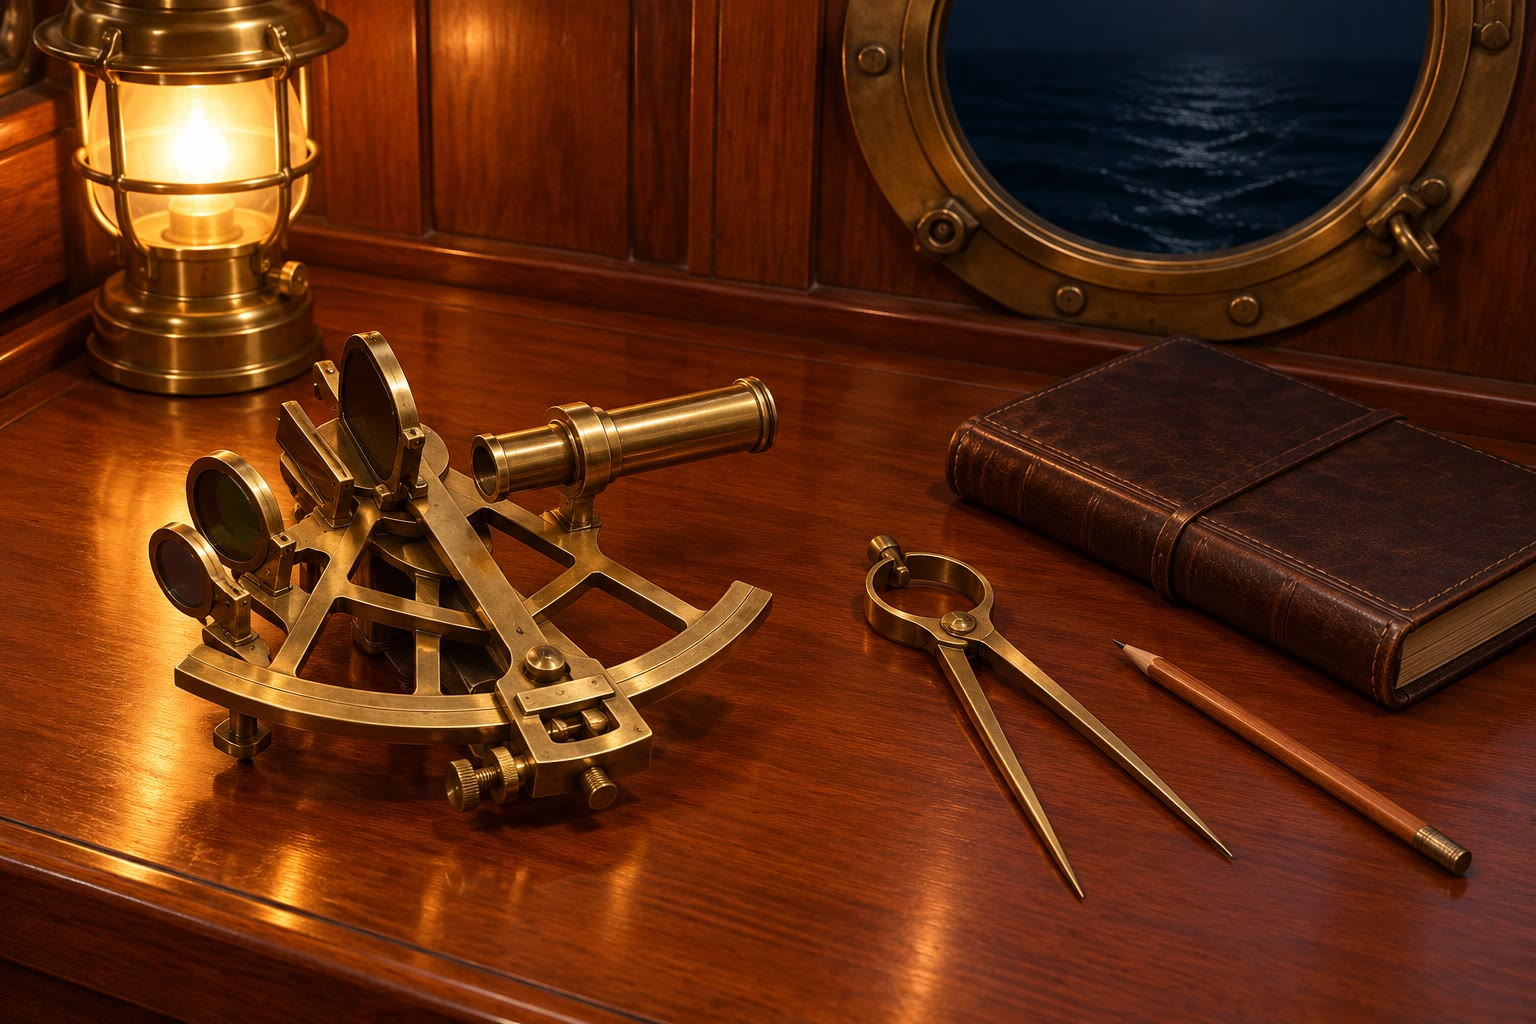
\includegraphics[width=0.55\linewidth]{images/book3/ai/b1-sextant.jpg}
\end{center}
\end{inthefield}

\section{Ejercicios}

\begin{exercise}[$\star$]\label{exo:b1:spherical-astronomy:1}
Un observador está a la \omterm{def:b1:spherical-astronomy:geographic}{latitud} \ang{52} N. ¿A qué \omterm{def:b1:spherical-astronomy:horizontal}{altura} se encuentra el \omterm{def:b1:spherical-astronomy:celestial-sphere}{polo
celeste} norte? ¿Qué estrellas, por su \omterm{def:b1:spherical-astronomy:equatorial}{declinación}, no se ponen nunca allí, y
cuáles no salen nunca?
\end{exercise}

\begin{exercise}[$\star$]\label{exo:b1:spherical-astronomy:2}
Conviértase una \omterm{def:b1:spherical-astronomy:equatorial}{ascensión recta} de \qty{6}{h}~\qty{45}{min} en grados. Con un
\omterm{def:b1:spherical-astronomy:sidereal-time}{tiempo sidéreo} local de \qty{10}{h}~\qty{0}{min}, ¿cuál es el \omterm{def:b1:spherical-astronomy:equatorial}{ángulo horario} de
una estrella de esa \omterm{def:b1:spherical-astronomy:equatorial}{ascensión recta}? ¿Está la estrella al este o al oeste del
meridiano?
\end{exercise}

\begin{exercise}[$\star$]\label{exo:b1:spherical-astronomy:3}
A la \omterm{def:b1:spherical-astronomy:geographic}{latitud} \ang{40} N, calcúlese la \omterm{def:b1:spherical-astronomy:horizontal}{altura} del Sol al mediodía en los dos
solsticios y en los equinoccios ($\varepsilon = \ang{23.44}$).
\end{exercise}

\begin{exercise}[$\star$]\label{exo:b1:spherical-astronomy:4}
¿Fue 1900 año bisiesto? ¿Lo fue 2000? ¿Lo será 2100? ¿En cuántos días por siglo
se desfasa el calendario juliano respecto de un \omterm{def:b1:spherical-astronomy:tropical-year}{año trópico} de 365.2422 días, y
en cuántos el gregoriano?
\end{exercise}

\begin{exercise}[$\star\star$]\label{exo:b1:spherical-astronomy:5}
Dos puntos están a la \omterm{def:b1:spherical-astronomy:geographic}{latitud} \ang{45} N, a las \omterm{def:b1:spherical-astronomy:geographic}{longitudes} \ang{0} y \ang{90} E.
Calcúlese la distancia sobre el \omterm{def:b1:spherical-astronomy:spherical-triangle}{círculo máximo} entre ellos ($R = \qty{6371}{km}$)
y la distancia a lo largo de su paralelo. ¿Cuál es más corta, y en cuánto?
\end{exercise}

\begin{exercise}[$\star\star$]\label{exo:b1:spherical-astronomy:6}
A la \omterm{def:b1:spherical-astronomy:geographic}{latitud} \ang{48} N, una estrella de \omterm{def:b1:spherical-astronomy:equatorial}{declinación} \ang{20} tiene el \omterm{def:b1:spherical-astronomy:equatorial}{ángulo
horario} \ang{30}. Calcúlese su \omterm{def:b1:spherical-astronomy:horizontal}{altura} y su \omterm{def:b1:spherical-astronomy:horizontal}{acimut}. ¿En qué dirección debe mirar
el observador?
\end{exercise}

\begin{exercise}[$\star\star$]\label{exo:b1:spherical-astronomy:7}
Calcúlese la duración del día a la \omterm{def:b1:spherical-astronomy:geographic}{latitud} \ang{60} N en el solsticio de junio,
tratando el Sol como un punto sobre un horizonte geométrico. Compruébese la
respuesta con la figura de la duración del día.
\end{exercise}

\begin{exercise}[$\star\star$]\label{exo:b1:spherical-astronomy:8}
Una estrella cruza el meridiano esta noche a las 22:00 hora solar media local.
¿A qué hora lo cruzará dentro de 30 días? ¿Dentro de cuántos días lo cruzará a
mediodía, cuando no es visible por la luz del día?
\end{exercise}

\begin{exercise}[$\star\star$]\label{exo:b1:spherical-astronomy:9}
Calcúlese la \omterm{def:b1:spherical-astronomy:insolation}{insolación} en el borde superior de la atmósfera al mediodía a la
\omterm{def:b1:spherical-astronomy:geographic}{latitud} \ang{45} N (a) en un equinoccio, tomando $r = a$; (b) en el solsticio de
junio, tomando para $r$ la distancia en el afelio. Datos: $S_0 = \qty{1361}{W.m^{-2}}$,
$a = \qty{149.598e6}{km}$, afelio \qty{152.100e6}{km}.
\end{exercise}

\begin{exercise}[$\star\star\star$]\label{exo:b1:spherical-astronomy:10}
Utilizando la \cref{prop:b1:spherical-astronomy:sun-declination}, calcúlense la
\omterm{def:b1:spherical-astronomy:equatorial}{declinación} y la \omterm{def:b1:spherical-astronomy:equatorial}{ascensión recta} del Sol cuando su longitud \omterm{def:b1:spherical-astronomy:ecliptic}{eclíptica} es
\ang{60}. ¿Cuántos grados va la \omterm{def:b1:spherical-astronomy:equatorial}{ascensión recta} por detrás de la longitud?
Explíquese con este resultado por qué la inclinación de la \omterm{def:b1:spherical-astronomy:ecliptic}{eclíptica} contribuye
a la \omterm{def:b1:spherical-astronomy:solar-time}{ecuación del tiempo}.
\end{exercise}

\begin{exercise}[$\star\star\star$]\label{exo:b1:spherical-astronomy:11}
Demuéstrese que en el solsticio de junio el Sol sale con un \omterm{def:b1:spherical-astronomy:horizontal}{acimut}
$\mathrm{A}_0$ tal que $\cos\mathrm{A}_0 = \sin\varepsilon/\cos\varphi$. ¿A qué
\omterm{def:b1:spherical-astronomy:geographic}{latitud} sale el Sol exactamente por el nordeste? ¿Qué ocurre con la fórmula a
\omterm{def:b1:spherical-astronomy:geographic}{latitudes} superiores a $\ang{90} - \varepsilon$?
\end{exercise}

\begin{exercise}[$\star\star\star$]\label{exo:b1:spherical-astronomy:12}
Un huso esférico es la parte de una esfera comprendida entre dos semicírculos
máximos que unen dos puntos opuestos, formando entre sí el ángulo $\theta$.
(a) Demuéstrese que su área es $2\theta R^2$. (b) Cada lado de un \omterm{def:b1:spherical-astronomy:spherical-triangle}{triángulo
esférico} $ABC$, prolongado hasta formar un \omterm{def:b1:spherical-astronomy:spherical-triangle}{círculo máximo} completo, da junto con
los otros dos pares de husos opuestos de ángulos $A$, $B$, $C$ que cubren la
esfera; el triángulo y su opuesto quedan cubiertos tres veces. Dedúzcase el
teorema de Girard: el área del triángulo es $R^2(A + B + C - \pi)$. (c)
Aplíquese al triángulo con tres ángulos rectos y al triángulo dibujado en este
capítulo (ángulos \ang{89.9}, \ang{64.9}, \ang{67.4}).
\end{exercise}

\section{Problema: una noche en un observatorio de montaña}

\begin{problem}[{Problema de fin de semana --- dónde está el Observatorio de Paranal,
qué muestra su cielo y cuánto dura su noche más larga}]
\label{pb:b1:spherical-astronomy:1}
% ledger: mpc:paranal, mpc:greenwich, simbad:sirius, simbad:canopus, usno:seasons-2026, earth:obliquity, usno:tropical-year
% numbers computed in the scratch calculator calc/ch01.py from the rounded data
El Observatorio de Paranal se encuentra en el desierto de Atacama, a la \omterm{def:b1:spherical-astronomy:geographic}{latitud}
\ang{24.63} S y la \omterm{def:b1:spherical-astronomy:geographic}{longitud} \ang{70.40} O. El Observatorio Real de Greenwich, por
el que se cuentan las \omterm{def:b1:spherical-astronomy:geographic}{longitudes}, está en \ang{51.48} N, \ang{0.00}. Dos estrellas
brillantes del cielo austral tienen las coordenadas
\begin{center}
\small
\begin{tabular}{lcc}
\hline
estrella & \omterm{def:b1:spherical-astronomy:equatorial}{ascensión recta} & \omterm{def:b1:spherical-astronomy:equatorial}{declinación} \\
\hline
Sirio & \qty{6}{h}~\qty{45}{min}~\qty{9}{s} & \ang{-16.72} \\
Canopo & \qty{6}{h}~\qty{23}{min}~\qty{57}{s} & \ang{-52.70} \\
\hline
\end{tabular}
\end{center}
Tómese $R = \qty{6371}{km}$, $\varepsilon = \ang{23.44}$, un \omterm{def:b1:spherical-astronomy:tropical-year}{año trópico} de
365.2422 días, y trátese el Sol como un punto sobre un horizonte geométrico.

\medskip
\noindent\textbf{Parte I --- Paranal sobre el globo.}
\begin{enumerate}
  \item Calcúlense las colatitudes de Paranal y de Greenwich, y su diferencia de
        longitud.
  \item Escríbase el teorema del coseno para el triángulo con vértices en el polo
        norte, Paranal y Greenwich, y calcúlese el coseno de la distancia angular
        $\Delta$ entre los dos observatorios.
  \item Dedúzcase $\Delta$ en grados y la distancia en kilómetros.
  \item Calcúlese el rumbo inicial desde Paranal hacia Greenwich
        (\cref{met:b1:spherical-astronomy:great-circle}).
  \item Compruébese el rumbo con el teorema del seno.
  \item ¿Llegaría a Greenwich un avión que mantuviera este rumbo durante todo el
        trayecto? Explíquese.
\end{enumerate}

\medskip
\noindent\textbf{Parte II --- El cielo de Paranal.}
\begin{enumerate}[resume]
  \item ¿A qué \omterm{def:b1:spherical-astronomy:horizontal}{altura} se encuentra el \omterm{def:b1:spherical-astronomy:celestial-sphere}{polo celeste} sur sobre el horizonte sur de
        Paranal?
  \item ¿A qué \omterm{def:b1:spherical-astronomy:horizontal}{altura} cruza Sirio el meridiano, y a qué lado del \omterm{def:b1:spherical-astronomy:celestial-sphere}{cenit}?
  \item ¿Por debajo de qué \omterm{def:b1:spherical-astronomy:equatorial}{declinación} es una \omterm{def:b1:spherical-astronomy:circumpolar}{estrella circumpolar} en Paranal?
        ¿Es Canopo circumpolar?
  \item ¿Cuál es la \omterm{def:b1:spherical-astronomy:horizontal}{altura} máxima que alcanza Canopo?
  \item Calcúlese el \omterm{def:b1:spherical-astronomy:equatorial}{ángulo horario} al que sale Sirio y el tiempo que permanece
        sobre el horizonte, en horas sidéreas.
  \item ¿A qué \omterm{def:b1:spherical-astronomy:horizontal}{acimut} sale Sirio?
\end{enumerate}

\medskip
\noindent\textbf{Parte III --- Relojes.}
\begin{enumerate}[resume]
  \item ¿Cuál es el \omterm{def:b1:spherical-astronomy:sidereal-time}{tiempo sidéreo} local cuando Sirio cruza el meridiano?
  \item Calcúlese la duración del día sidéreo, y en cuántos minutos se adelanta
        cada noche el paso de una estrella por el meridiano.
  \item Tómese el \omterm{def:b1:spherical-astronomy:sidereal-time}{tiempo sidéreo} local a la medianoche local media igual a
        \qty{12}{h} en el equinoccio de marzo (20 de marzo de 2026), cuando el Sol
        está cerca del \omterm{def:b1:spherical-astronomy:ecliptic}{punto vernal}; entonces gana $24/365.2422$ horas cada día.
        ¿Cuántos días después del equinoccio cruza Sirio el meridiano a la
        medianoche local media? ¿En qué fecha?
  \item Esa noche, ¿en cuánto difiere la hora solar media en Paranal de la hora
        de Greenwich?
  \item La \omterm{def:b1:spherical-astronomy:solar-time}{ecuación del tiempo} es entonces de unos \qty{-3}{min}. ¿Qué hora marca
        un reloj de sol en el observatorio (\omterm{def:b1:spherical-astronomy:solar-time}{tiempo solar aparente}) cuando Sirio
        cruza el meridiano?
  \item ¿Cuánto antes lo cruza una semana después?
\end{enumerate}

\medskip
\noindent\textbf{Parte IV --- La noche más larga.}
\begin{enumerate}[resume]
  \item ¿Cuál es la \omterm{def:b1:spherical-astronomy:equatorial}{declinación} del Sol en cada solsticio?
  \item Calcúlese la \omterm{def:b1:spherical-astronomy:horizontal}{altura} del Sol al mediodía en Paranal en los solsticios de
        junio y de diciembre. ¿A qué lado del \omterm{def:b1:spherical-astronomy:celestial-sphere}{cenit} está en diciembre?
  \item En el solsticio de diciembre la distancia Sol--Tierra es 0.9837 veces la
        distancia media. Calcúlese la \omterm{def:b1:spherical-astronomy:insolation}{insolación} al mediodía en el borde superior
        de la atmósfera sobre Paranal ($S_0 = \qty{1361}{W.m^{-2}}$).
  \item ¿En qué solsticio es más larga la noche en Paranal? Calcúlese el \omterm{def:b1:spherical-astronomy:equatorial}{ángulo
        horario} de la puesta en esa fecha.
  \item ¿A qué \omterm{def:b1:spherical-astronomy:horizontal}{acimut} sale el Sol en esa fecha?
  \item Dedúzcase la duración de la noche más larga del año en Paranal, en horas
        y minutos.
\end{enumerate}
\end{problem}
